\subsection{\label{subsec:FZV6}Konfokales Mikroskop}
\textbf{\textit{Erklären Sie den Aufbau eines konfokalen Mikroskops. Welche Aufgabe hat das Pinhole?}} \\
$\rightarrow$
Die Antwort auf die vorherige Frage \ref{subsec:FZV5} deutet darauf hin, dass es für die Einzelmolekülspektroskopie 
erforderlich ist, einen einzelnen Fluorophor in einem äußerst kleinen Probenvolumen vorzubereiten, 
um das Signal im Vergleich zu Störsignalen, insbesondere Streulicht, aufzulösen. 
Um die hohen Anforderungen an die Probenherstellung zu umgehen, bietet die konfokale Fluoreszenzmikroskopie 
eine alternative Methode. Die schematische Darstellung eines konfokalen Mikroskops 
in Abb.~\ref{fig:convocal} zeigt die Funktionsweise dieses Verfahrens.
\begin{figure}[h!]
    \centering
    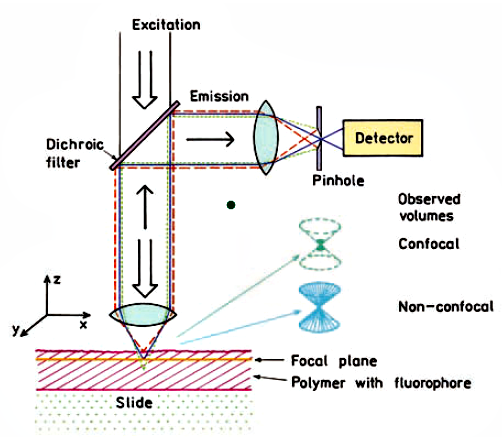
\includegraphics[width=0.7\textwidth]{ConvocalNeu.png}
    \caption{\label{fig:convocal}Schematischer Aufbau eines konfokalen Mikroskops.
    Die Funktionsweise und alle relevanten optischen Bauteile sind im Haupttext beschrieben.
    Die Graphik wurde Ref.~\cite{Prinzip} entnommen.}
\end{figure}\FloatBarrier
Zunächst passiert das Anregungslicht (\textit{Excitation}, dicker Pfeil) einen dichroitischen Spiegel 
(\textit{Dichroic filter}), der als wellenlängenabhängiger Strahlteiler fungiert. 
Das höher energetische Anregungslicht passiert den Spiegel ungehindert, während das emittierte 
energieärmere Licht (\textit{Emission}, dünner Pfeil) des Fluorophors reflektiert wird. 
Hierdurch wird zunächst ermöglicht, dass nur Licht einer bestimmten Wellenlänge den Detektor 
erreicht, was das Signal vom Anregungslicht befreit und so auflösbar macht. \\
Das Licht der Anregungsquelle (z.B. Diodenlaser) wird in negativer z-Richtung mithilfe einer Linse 
auf eine Polymerschicht mit eingebundenen Fluorophoren fokussiert. Das von der beleuchteten 
Probenschicht zurückgestrahlte Licht (Fluoreszenz, Verunreinigungen, Raman-Lichtstreuung) wird 
über den Spiegel in x-Richtung auf einen Detektor fokussiert. Ein entscheidender Bestandteil, 
der das detektierte Probenvolumen minimiert, ist die Lochblende (\textit{Pinhole}). 
Diese Blende lässt bei richtiger Justage nur einen kleinen Teil des Lichts zum Detektor passieren, 
womit das Licht aus der Fokusebene (\textit{Focal plane}) untersucht werden kann. 
Anhand der unterschiedlich eingezeichneten Strahlengänge kann man den Einfluss der Lochblende 
erkennen, was durch den Vergleich der untersuchten Volumen (\textit{Observed volumes}) auf 
der rechten Seite der Abbildung verdeutlicht wird. Die Reduzierung des untersuchten Volumens 
ermöglicht zum einen die getrennte Betrachtung einzelner Moleküle und verringert das Störsignal 
der Raman-Streuung erheblich. \\
Insgesamt ist die Kombination aus Lochblende und einem dichroitischen Spiegel das Erfolgskonzept 
der konfokalen Mikroskopie. Durch beide Komponenten wird das Signal-Rausch-Verhältnis erheblich 
verbessert, was letztendlich die Detektion des Fluoreszenzsignals einzelner Moleküle ermöglicht \cite{Prinzip}. \\

